\documentclass[11pt,a4paper]{article}
\usepackage[margin=2.5cm]{geometry}
\usepackage{amsmath,amssymb,amsthm,booktabs,graphicx,hyperref,xcolor,array,caption,authblk,microtype,enumitem}
\captionsetup{font=small,labelfont=bf}
\newtheorem{proposition}{Proposition}
\newtheorem{lemma}{Lemma}
\theoremstyle{remark}\newtheorem{remark}{Remark}
\newcommand{\R}{\mathbb{R}}
\DeclareMathOperator{\softmax}{softmax}
\DeclareMathOperator{\erank}{erank}
\graphicspath{{./}}

\title{\textbf{Statistical auditing of trained neural networks: exact coverage of bootstrap-replicate intervals, multiplicity-controlled neuron tests, and the low-rank structure of hidden layers}}
\author[1]{Mohamad Yamen Al-Mohamad}
\author[1,*]{Ali Akbar Hydari}
\author[1]{Hossein Jabbari Khamnei}
\author[2]{Mehrdad Lakestani}
\affil[1]{Department of Statistics, University of Tabriz, Tabriz, Iran}
\affil[2]{Department of Applied Mathematics, University of Tabriz, Tabriz, Iran}
\affil[*]{Corresponding author: heydari@tabrizu.ac.ir}
\date{}

\begin{document}
\maketitle

\begin{abstract}
\noindent Statistical tools are increasingly used to ``audit'' a trained network: confidence intervals for its accuracy, hypothesis tests for hidden neurons, logistic surrogates of its output layer, and simplification of its architecture. We study which of these procedures keep their nominal statistical properties, for a network viewed as a fixed feature map followed by an affine--softmax head. Our main result is an \emph{exact} coverage law for the popular ``CLT interval'' computed from $B$ bootstrap replicates of accuracy: its coverage of the true accuracy converges to $2F_{B-1}\!\big(t_{B-1,1-\alpha/2}/\sqrt{B+1}\big)-1$, where $F_{B-1}$ is the $t$ distribution function; this is $28\%$ for $B=30$ and $5\%$ for $B=1000$ at the nominal $95\%$ level, irrespective of the sample size. Simulations match the law. Second, we show that testing neurons at raw levels is unreliable (at least one false discovery in $84$--$89\%$ of null families of 40 neurons), that retraining-bootstrap schemes that reuse the full-data fit are optimistic, and that per-neuron inference is weakly identified because trained hidden layers have very low effective rank: $2$--$2.5$ for $10$--$16$ units in two classical data sets, $7.6$ of $64$ units in a three-hidden-layer network and $11.4$ of $128$ in a CNN trained on MNIST images, where on average $0$ and $1$ neurons respectively have a significant individual ablation effect. Third, the same low rank explains why reconstruction-based pruning works. We show that sequential Optimal Brain Surgeon on the last layer \emph{equals} the least-squares compensated head of the kept set, that ThiNet's rescaling is a restriction of it, and we give a pivoted-QR selection rule with an exact Frobenius error bound; in experiments against ThiNet, OBS, neuron merging, CUR and magnitude pruning on five tabular data sets and two PyTorch image models, compensated pruning keeps accuracy within $0.4$ points at a quarter of the width of a CNN, where uncompensated or weakly compensated rules lose $2$--$17$ points. We do not claim novelty of the compensation itself; our contribution is the statistical analysis that quantifies when the audit is valid and why the network can be compressed. All procedures are in the open-source Python package \texttt{annstat}.
\medskip

\noindent\textbf{Keywords:} neural networks; confidence intervals; bootstrap; multiple testing; model compression; effective rank; explainable AI
\end{abstract}

\section{Introduction}
Neural networks are accurate but opaque. Besides post-hoc explanation tools such as SHAP and LIME \cite{lundberg2017,ribeiro2016}, a statistical line of work asks whether the \emph{components} of a trained network can be examined with the usual inferential machinery: intervals for performance \cite{white2001}, significance tests for inputs and hidden neurons \cite{horel2020,olden2002}, interpretable surrogates of the output layer, and simplification of the architecture by pruning \cite{blalock2020,hoefler2021}. A recent proposal in this direction \cite{almohamad2024} combines (a) bootstrap and CLT intervals for accuracy, (b) Mann--Whitney tests of the contribution of each hidden neuron to each output, (c) logistic regression on the hidden-layer outputs and (d) reduction of the hidden layer by clustering or principal components.

Such audits carry two risks. First, the inferential statements may be wrong even though each step looks reasonable: an interval built from bootstrap replicates may have little to do with the uncertainty of the accuracy, and a family of $k\binom q2$ neuron tests at level $0.05$ is certain to produce false positives. Second, the structure of the object being audited can make the questions ill posed: if the hidden layer is nearly low-rank, individual neurons are not identified and a per-neuron significance statement carries little information.

\paragraph{Contributions.} The paper has one theme -- \emph{when is a statistical audit of a trained network valid, and what does the audit reveal about the network} -- and three results.
\begin{enumerate}[leftmargin=*,itemsep=1pt]
\item \textbf{An exact coverage law} for the CLT-of-replicates interval (Proposition~\ref{prop:clt}), with a complete proof, confirmed by simulation, together with a comparison with Wilson, Clopper--Pearson and bootstrap intervals, and an assessment of retraining-bootstrap schemes (Sections~\ref{sec:e1}--\ref{sec:e2}).
\item \textbf{Multiplicity-controlled neuron inference and its limits}: paired and independent contrast tests, association tests, paired-bootstrap ablation tests, and a drop-one likelihood-ratio test for the surrogate; simulations of the false-discovery problem and evidence from classical and deep networks that hidden layers have very low effective rank, so that per-neuron inference is weakly identified (Sections~\ref{sec:e3},\ref{sec:e5},\ref{sec:e7}).
\item \textbf{A statistical explanation of why pruning works.} We show that sequential Optimal Brain Surgeon (OBS), the least-squares ``compensated'' head and the reconstruction step of ThiNet are nested instances of one least-squares problem (Proposition~\ref{prop:equiv}); give an exact Frobenius error bound for a pivoted-QR selection (Proposition~\ref{prop:bound}); and compare against published baselines on tabular and image data (Sections~\ref{sec:e6}--\ref{sec:e8}). The compensation idea is not new; we make no claim to the contrary (Section~\ref{sec:related}).
\end{enumerate}
We also release the methods as the Python package \texttt{annstat}.

\section{Related work}\label{sec:related}
\paragraph{Inference for neural networks.} White and Racine \cite{white2001} developed bootstrap inference for neural-network regression; Horel and Giesecke \cite{horel2020} proposed significance tests for inputs; connection-weight methods \cite{garson1991,olden2002} and permutation importance \cite{breiman2001,fisher2019} address variable importance, with well-known extrapolation problems under dependence \cite{hooker2021}. Knockoffs \cite{candes2018} and conditional-independence tests \cite{shah2020} give population-level alternatives. For predictive uncertainty, conformal prediction provides distribution-free guarantees \cite{lei2018,angelopoulos2023}.
\paragraph{Estimating and comparing performance.} The uncertainty of a generalisation estimate is subtle: there is no unbiased estimator of the variance of $K$-fold cross-validation \cite{bengio2004}, naive resampled $t$-tests are invalid \cite{nadeau2003,dietterich1998}, and cross-validation intervals target the average over training sets rather than the fitted model \cite{bates2023}. For a \emph{fixed} classifier, accuracy on i.i.d.\ test cases is binomial and Wilson/Clopper--Pearson intervals apply \cite{wilson1927,clopper1934,brown2001,agresti1998}; the bootstrap \cite{efron1979,efron1997,davison1997} is an alternative. Multiple comparisons across data sets are treated in \cite{demsar2006,benavoli2017}.
\paragraph{Multiplicity.} Holm \cite{holm1979}, Benjamini--Hochberg \cite{benjamini1995} and Benjamini--Yekutieli \cite{benjamini2001} are the standard family-wise and false-discovery controls; classical rank tests are \cite{mann1947,wilcoxon1945,kruskal1952,friedman1937}. Wald tests in logistic models fail under separation \cite{hauck1977,albert1984} (remedies in \cite{firth1993}).
\paragraph{Pruning and compression.} Early second-order criteria are Optimal Brain Damage \cite{lecun1990} and Optimal Brain Surgeon \cite{hassibi1993}; layer-wise OBS was revived in \cite{dong2017} and scaled in \cite{frantar2022,frantar2023}, where weight updates reconstruct the layer's output on calibration data. Structured methods include magnitude/filter pruning \cite{han2015,li2017}, Taylor criteria \cite{molchanov2017,molchanov2019}, channel pruning by LASSO and least squares \cite{he2017}, ThiNet \cite{luo2017} (greedy channel selection with least-squares reconstruction), data-free merging of similar neurons \cite{srinivas2015,kim2020}, convex formulations \cite{aghasi2017} and the lottery-ticket line \cite{frankle2019}. The low-rank structure of weights and representations has been documented repeatedly \cite{denil2013,raghu2017,kornblith2019,ansuini2019,aghajanyan2021,hu2022}; our contribution here is to connect it to inferential identifiability and to the error of compensated pruning. On the numerical side, subset selection by rank-revealing QR \cite{businger1965,gu1996}, CUR decompositions \cite{mahoney2009} and Nystr\"om approximations \cite{williams2001} select actual columns of a matrix with approximation guarantees.

\paragraph{Position of the present work.} Reconstruction-based compensation of removed units by least squares is therefore established. What we add is (i)~the exact identification of OBS with the full least-squares compensation, so that the \emph{selection rule} is the only difference between these methods; (ii)~a label- and head-free selector with an exact Frobenius bound; (iii)~empirical evidence that low effective rank, which also limits per-neuron inference, is what makes the compensation effective.

\section{Setting and notation}
A feed-forward network with $L$ hidden layers computes $f(x)=g\!\left(W^\top\varphi(x)+b\right)$, where $\varphi:\R^d\to\R^k$ is the post-activation map of the \emph{last} hidden layer, $W\in\R^{k\times q}$, $b\in\R^q$, and $g=\softmax$ (classification, $q$ classes; binary single-logit heads are symmetrised to $(-z/2,z/2)$) or the identity (regression). All analyses use only $\varphi$, $(W,b)$ and, where stated, a refitting routine, so they are independent of the training framework. For a sample $x_1,\dots,x_n$ let $H\in\R^{n\times k}$ be the matrix of hidden activations. A neuron is \emph{dead on the sample} if its column is constant. The \emph{effective rank} is $\erank(H)=\exp(-\sum_i p_i\log p_i)$, $p_i=\lambda_i/\sum_l\lambda_l$ for the eigenvalues $\lambda_i$ of the activation covariance \cite{roy2007}; $1\le\erank\le k$. The \emph{participation ratio} is $(\sum\lambda_i)^2/\sum\lambda_i^2$. $Z=HW+\mathbf 1b^\top$ denotes the logits.

\section{Methods}\label{sec:methods}
\subsection{Intervals for accuracy}\label{sec:ci}
Let $\theta$ be the population accuracy of the \emph{fixed} trained network. On $n$ i.i.d.\ test cases the number of hits is $\mathrm{Bin}(n,\theta)$, which gives Wilson and Clopper--Pearson intervals, or percentile/basic bootstrap intervals from resampled test cases (without retraining). To reflect training variability one may retrain on bootstrap samples; we distinguish \emph{own-sample} scoring, \emph{out-of-bag} (OOB) scoring after a warm start from the full-data fit, and OOB scoring after a cold start (re-initialisation). The ``CLT interval'' of \cite{almohamad2024} is $\bar a\pm t_{B-1,1-\alpha/2}\,s/\sqrt B$ with $\bar a,s$ the mean and standard deviation of $B$ replicates of accuracy.

\begin{proposition}[Exact asymptotic coverage of the CLT-of-replicates interval]\label{prop:clt}
Let $\theta\in(0,1)$, $\hat p=X/n$ with $X\sim\mathrm{Bin}(n,\theta)$, and, given $\hat p$, let $a_b=Y_b/n$ with $Y_1,\dots,Y_B$ i.i.d.\ $\mathrm{Bin}(n,\hat p)$, $B\ge2$ fixed. Let $\bar a,s$ be the mean and sample standard deviation of $a_1,\dots,a_B$ and $I=\bar a\pm t_{B-1,1-\alpha/2}\,s/\sqrt B$. Then as $n\to\infty$
\[
\Pr(\theta\in I)\;\longrightarrow\;2F_{B-1}\!\left(\frac{t_{B-1,1-\alpha/2}}{\sqrt{B+1}}\right)-1,
\]
$F_{B-1}$ being the distribution function of Student's $t_{B-1}$. The limit tends to $0$ as $B\to\infty$.
\end{proposition}
The proof (Appendix~\ref{app:proofs}) rests on the fact that $\hat p-\theta$ and $\bar a-\hat p$ are independent contributions to the error of $\bar a$, whereas $s/\sqrt B$ measures only the second. For $\alpha=0.05$ the limits are $0.914,0.680,0.488,0.284,0.156,0.049$ for $B=2,5,10,30,100,1000$. The interval is a confidence interval for the bootstrap mean, i.e.\ for $\hat p$ (and then of nearly zero width), not for $\theta$. A direct consequence is that increasing $B$, which usually improves a Monte-Carlo approximation, makes this interval \emph{worse} as an interval for $\theta$.

\subsection{Tests for hidden neurons}
\paragraph{Contribution tests.} The contribution of neuron $i$ to logit $j$ is $c_{i\cdot j}=h_{\cdot i}\,w_{ij}$. Columns $j,j'$ are computed on the \emph{same} $n$ samples, so a paired test (Wilcoxon signed-rank; Friedman omnibus for $q\ge3$) is appropriate; independent-sample tests (Mann--Whitney, Kruskal--Wallis) are kept for reproducibility. Rank-biserial effect sizes are reported, and the $k\binom q2$ p-values are adjusted (Holm for pairs, Benjamini--Hochberg for omnibus tests).
\paragraph{Association tests.} Per neuron: Kruskal--Wallis across classes (effect size $\varepsilon^2=H/(n-1)$ \cite{tomczak2014}) or Spearman correlation with the response, BH-adjusted.
\paragraph{Ablation tests.} Let $d_i=\ell_i^{(-j)}-\ell_i$ be the per-sample loss increase when neuron $j$ is set to $0$. A paired bootstrap gives a confidence interval for $\mathbb E d$ and the one-sided p-value $(1+\#\{\bar d^*\le0\})/(B+1)$, BH-adjusted; a minimum effect size can be required.
\paragraph{Input tests.} Permuting input $x_j$ $R$ times gives the p-value $(1+\#\{\text{loss}^*\le\text{loss}_0\})/(R+1)$: a model-reliance test of the \emph{fitted} network \cite{breiman2001,fisher2019}, subject to the extrapolation caveat of \cite{hooker2021}.

\subsection{Surrogate head and drop-one likelihood-ratio tests}
Refitting the output layer by maximum likelihood on activations gives a multinomial logit with Wald standard errors, a likelihood-ratio test of the whole layer, McFadden $R^2$, AIC and BIC. Wald tests are unreliable under (quasi-)separation and collinearity \cite{hauck1977,albert1984}, typical for a network that fits its training data. We therefore add a \emph{drop-one likelihood-ratio test} per neuron ($\chi^2_{q-1}$, BH-adjusted).

\subsection{Low rank and compensated width reduction}\label{sec:lsc}
Let $S$ be a set of $m<k$ kept neurons and $P$ the removed ones. \emph{Compensated pruning} keeps $H_S$ and replaces the head by the least-squares fit of the full logits on $[\mathbf 1\;H_S]$:
\begin{equation}\label{eq:lsc}
W'=W_S+\hat B_S W_P,\qquad b'=b+W_P^\top\hat B_0,\qquad [\hat B_0;\hat B_S]=(A^\top A)^{-1}A^\top H_P,\ A=[\mathbf 1\;H_S].
\end{equation}
(We call this LSC.) Only the $m$ kept neurons are computed at inference. Cluster and PCA reductions \cite{almohamad2024}, in contrast, build every new feature from all $k$ neurons: they shrink the head but not the number of neurons evaluated.

\begin{proposition}[Unification: OBS, LSC and ThiNet's reconstruction]\label{prop:equiv}
Let $A_k=[\mathbf 1\;H]$ have full column rank, $G=A_k^\top A_k$ and $\Theta_0=[b^\top;W]$, so $Z=A_k\Theta_0$. (a)~For any removal order, sequential layer-wise OBS on the loss $\|A_k(\Theta-\Theta_0)\|_F^2$ with exact Hessian $G$, removing one neuron at a time with the OBS update, ends at $\Theta'=[b'^\top;W']$ of \eqref{eq:lsc} for the final kept set $S$; so OBS and LSC differ only through the \emph{selection} of $S$. (b)~$\Theta'$ is the unique minimiser of $\|Z-H_S\Theta_W-\mathbf 1\Theta_b^\top\|_F^2$ over all affine heads on the kept neurons. (c)~ThiNet's final step, a per-neuron rescaling $W_S\mapsto\mathrm{diag}(s)W_S$ with $b$ fixed, minimises the same loss over a subset of these heads; hence on the same kept set its logit error is never smaller than that of LSC.
\end{proposition}

\begin{proposition}[Exact error bound for pivoted-QR selection]\label{prop:bound}
Let $Z'$ be the logits of the compensated network with kept set $S$ and let $R=H_P-A\hat B$. Then $Z-Z'=RW_P$ and $\|Z-Z'\|_F\le\|W_P\|_2\,\|R\|_F$. If $S$ is the set of the first $m$ pivots of a column-pivoted QR factorisation $\tilde H P=QR_Q$ of the centred activations $\tilde H=H-\mathbf 1\bar h^\top$, where $R_Q$ is upper triangular with leading $m\times m$ block $R_{11}$, off-diagonal block $R_{12}$ and trailing block $R_{22}$, then $\|R\|_F=\|R_{22}\|_F$ exactly, and $\|R_{22}\|_F^2\ge\sum_{i>m}\sigma_i^2(\tilde H)$. For a strong rank-revealing QR with parameter $f\ge1$ \cite{gu1996}, $\|R_{22}\|_F^2\le(1+f^2m(k-m))\sum_{i>m}\sigma_i^2(\tilde H)$.
\end{proposition}
\noindent Thus the in-sample logit error of compensated pruning is controlled by the tail of the singular values of the centred activation matrix -- the spectrum whose decay is measured by the effective rank. (Plain LAPACK pivoting, used in the package, carries no worst-case guarantee of the last kind; Section~\ref{sec:e8} reports how close it comes in practice.)

\section{Software}
The methods are implemented in the open-source Python package \texttt{annstat} (NumPy, SciPy, pandas, scikit-learn, Matplotlib). A thin \texttt{ModelAdapter} exposes $\varphi$ (for any hidden layer), the head $(W,b)$ and an optional refit routine; adapters exist for scikit-learn MLPs and, through hooks and callables, for PyTorch (used in Section~\ref{sec:e7}) and Keras (not executed in our environment). \texttt{StatisticalTuner.analyze} returns performance intervals, neuron tests, redundancy diagnostics, input tests, the surrogate and a reduction path. The module \texttt{annstat.baselines} contains our reimplementations of ThiNet, layer-wise OBS, data-free neuron merging, CUR-leverage selection and magnitude pruning for a single hidden layer; they follow the cited ideas and are not ports of the original code bases. The test suite (22 tests) includes the identity of Proposition~\ref{prop:equiv}(a) and the bound of Proposition~\ref{prop:bound}.

\section{Experiments}
All code is in \texttt{experiments/}; every table is generated from stored results.

\subsection{E1: coverage of accuracy intervals}\label{sec:e1}
The hit indicator of a fixed network on i.i.d.\ data is Bernoulli$(\theta)$, so coverage depends only on $(\theta,n)$ and can be simulated exactly: $\theta\in\{0.8,0.9,0.95,0.99\}$, $n\in\{30,100,300,1000\}$, $5000$ replicates, $B=1000$ bootstrap draws.
\begin{table}[ht]\centering\small
\caption{Empirical coverage (nominal $0.95$) of intervals for the accuracy of a fixed classifier, $\theta=0.90$; last column: mean width at $n=100$.}\label{tab:e1}
\begin{tabular}{lrrrrr}\toprule
Method & $n=30$ & $n=100$ & $n=300$ & $n=1000$ & width ($n{=}100$)\\\midrule
Wald & 0.807 & 0.928 & 0.935 & 0.951 & 0.115\\
Wilson & 0.979 & 0.933 & 0.956 & 0.945 & 0.117\\
Clopper-Pearson & 0.994 & 0.953 & 0.964 & 0.953 & 0.125\\
Bootstrap percentile & 0.953 & 0.954 & 0.953 & 0.950 & 0.114\\
Bootstrap, basic (Alg.~7 of \cite{almohamad2024}) & 0.807 & 0.925 & 0.940 & 0.949 & 0.114\\
CLT of replicates, $B=30$ (Alg.~6) & 0.258 & 0.279 & 0.275 & 0.281 & 0.022\\
CLT of replicates, $B=1000$ (Alg.~6) & 0.217 & 0.134 & 0.065 & 0.049 & 0.004\\
\bottomrule\end{tabular}

\end{table}
Wilson, Clopper--Pearson and the percentile bootstrap are close to nominal from moderate $n$ (Clopper--Pearson is conservative); Wald and basic bootstrap under-cover at small $n$ and near the boundary (Table~\ref{tab:e1b}, $\theta=0.99$). The CLT-of-replicates interval has coverage $0.28$ ($B=30$) and $0.049$ ($B=1000$) at $n=1000$, against the limits $0.284$ and $0.049$ of Proposition~\ref{prop:clt}; a separate simulation at $n=20{,}000$ ($4000$ replicates) gives $0.290$ and $0.053$. Its mean width at $n=100$ is $0.022$ and $0.004$, against $\approx0.115$ for the valid intervals.
\begin{table}[ht]\centering\small
\caption{As Table~\ref{tab:e1} for $\theta=0.99$.}\label{tab:e1b}
\begin{tabular}{lrrrrr}\toprule
Method & $n=30$ & $n=100$ & $n=300$ & $n=1000$ & width ($n{=}100$)\\\midrule
Wald & 0.259 & 0.628 & 0.788 & 0.932 & 0.025\\
Wilson & 0.960 & 0.918 & 0.964 & 0.966 & 0.051\\
Clopper-Pearson & 0.996 & 0.981 & 0.986 & 0.977 & 0.052\\
Bootstrap percentile & 0.259 & 0.628 & 0.950 & 0.959 & 0.026\\
Bootstrap, basic (Alg.~7 of \cite{almohamad2024}) & 0.260 & 0.627 & 0.791 & 0.935 & 0.026\\
CLT of replicates, $B=30$ (Alg.~6) & 0.001 & 0.351 & 0.252 & 0.292 & 0.006\\
CLT of replicates, $B=1000$ (Alg.~6) & 0.000 & 0.354 & 0.201 & 0.127 & 0.001\\
\bottomrule\end{tabular}

\end{table}
\begin{figure}[ht]\centering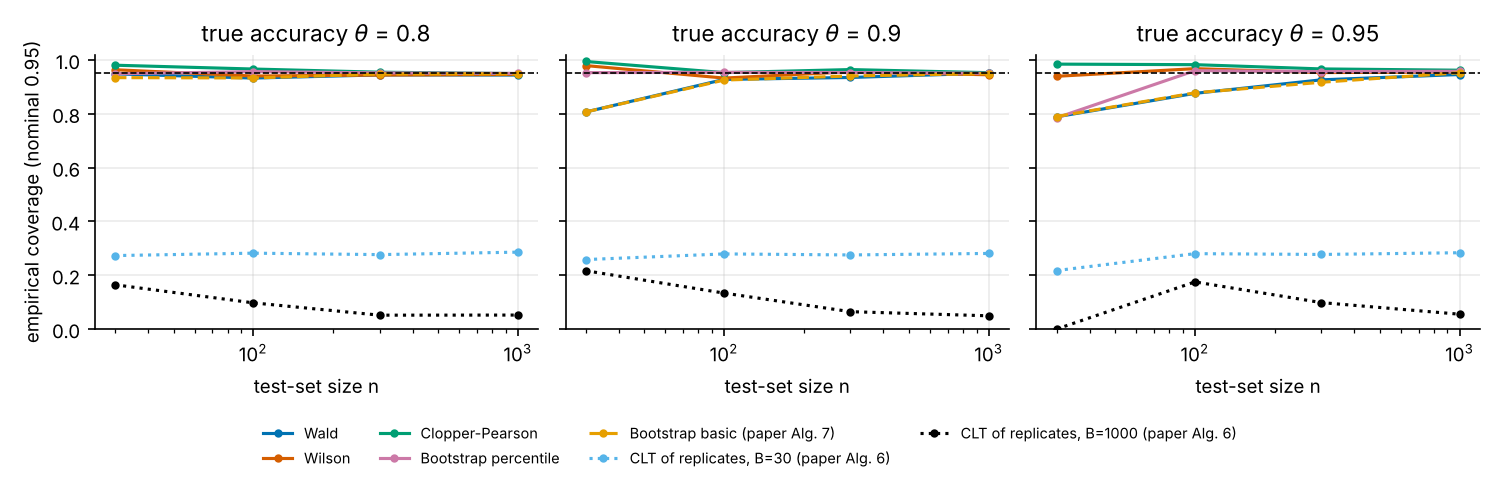
\includegraphics[width=\textwidth]{e1_coverage.png}
\caption{Coverage versus test-set size. The CLT-of-replicates intervals (dotted) are far below nominal and do not improve with $n$.}\label{fig:e1}\end{figure}

\subsection{E2: bootstrap schemes with retraining}\label{sec:e2}
For Iris, Wine and Breast Cancer (one hidden layer, $k=10,16,16$; 70/30 split) we retrained the network on $150$ stratified bootstrap samples ($60$ for the cold-start scheme) and scored it under the schemes of Section~\ref{sec:ci}.
\begin{table}[ht]\centering\small
\caption{Retraining-bootstrap accuracy: percentile 95\% intervals of the replicates; last row of each block: Wilson interval of the held-out accuracy of the original network.}\label{tab:e2}
\begin{tabular}{llrr}\toprule
Data set & Quantity & Estimate & 95\% interval\\\midrule
iris & own-sample, warm start (paper Alg.7) & 0.972 & [0.933, 1.000]\\
iris & out-of-bag, warm start & 0.948 & [0.881, 1.000]\\
iris & out-of-bag, cold start & 0.931 & [0.859, 0.975]\\
iris & hold-out accuracy (Wilson) & 1.000 & [0.921, 1.000]\\
\midrule
wine & own-sample, warm start (paper Alg.7) & 1.000 & [1.000, 1.000]\\
wine & out-of-bag, warm start & 0.990 & [0.955, 1.000]\\
wine & out-of-bag, cold start & 0.959 & [0.910, 1.000]\\
wine & hold-out accuracy (Wilson) & 0.981 & [0.902, 0.997]\\
\midrule
breast cancer & own-sample, warm start (paper Alg.7) & 0.994 & [0.982, 1.000]\\
breast cancer & out-of-bag, warm start & 0.989 & [0.972, 1.000]\\
breast cancer & out-of-bag, cold start & 0.978 & [0.947, 1.000]\\
breast cancer & hold-out accuracy (Wilson) & 0.953 & [0.910, 0.976]\\
\bottomrule\end{tabular}

\end{table}
The mean accuracy decreases from own-sample to warm-start OOB to cold-start OOB in all three data sets (Iris $0.972\to0.948\to0.931$; Wine $1.000\to0.990\to0.959$; Breast Cancer $0.994\to0.989\to0.978$): own-sample evaluation scores a model on its own training data and a warm-started model has already seen the out-of-bag points. Only the cold-start scheme gives a clean out-of-sample estimate, whose target (a network trained on $\approx63\%$ of the pool) differs from that of a single hold-out split.

\subsection{E3: multiplicity}\label{sec:e3}
We simulated $k=50$ neurons, $10$ differing between $3$ classes (shift $0.5$ per class index) and $40$ null, tested by Kruskal--Wallis, $400$ replicates.
\begin{table}[ht]\centering\small
\caption{Raw $p<0.05$ versus Holm / Benjamini--Hochberg adjustment (40 null, 10 non-null neurons).}\label{tab:e3}
\begin{tabular}{rrrrrrr}\toprule
$n$ & P(any FP) raw & P(any FP) Holm & FDR raw & FDR BH & power raw & power BH\\\midrule
60 & 0.860 & 0.020 & 0.193 & 0.035 & 0.766 & 0.380\\
150 & 0.835 & 0.052 & 0.147 & 0.038 & 0.994 & 0.968\\
300 & 0.890 & 0.058 & 0.159 & 0.043 & 1.000 & 1.000\\
\bottomrule\end{tabular}

\end{table}
Unadjusted testing yields at least one false positive in $84$--$89\%$ of families (theory $1-0.95^{40}=0.87$) and a false-discovery proportion of $15$--$19\%$. Holm brings the family-wise error to $0.02$--$0.06$ and BH the FDR to $0.035$--$0.043$, at a power cost that is large only in the smallest sample ($0.77\to0.38$ at $n=60$; $0.99\to0.97$ at $n=150$).

\subsection{E5: case studies on classical data}\label{sec:e5}
We audited a network with $k=10$ neurons on Iris (80/20 split, test $n=30$) and $k=16$ on Breast Cancer (70/30, test $n=171$); both use a single split.
\begin{table}[ht]\centering\small
\caption{Case-study summary produced by \texttt{StatisticalTuner}.}\label{tab:e5}
\begin{tabular}{lrr}\toprule
 & Iris ($k{=}10$) & Breast cancer ($k{=}16$)\\\midrule
Test accuracy (Wilson 95\% CI) & 0.967 [0.833, 0.994] & 0.971 [0.933, 0.987]\\
Bootstrap percentile 95\% CI & [0.900, 1.000] & [0.947, 0.994]\\
Effective rank of hidden layer & 2.02 of 10 & 2.50 of 16\\
Neurons associated with response (BH) & 10 / 10 & 16 / 16\\
Neurons with significant ablation effect & 3 / 10 & 4 / 16\\
Pairwise contrasts: Mann--Whitney raw / Holm & 18 / 16 of 30 & n/a (binary)\\
Pairwise contrasts: Wilcoxon raw / Holm & 30 / 30 of 30 & n/a (binary)\\
Surrogate McFadden $R^2$ & 0.979 & 0.974\\
Surrogate LR test, whole layer ($p$) & 2.6e-43 & 1.2e-98\\
Neurons significant, Wald ($p<.05$, raw) & 0 / 10 & 0 / 16\\
Neurons significant, drop-one LR (BH) & 0 / 10 & 1 / 16\\
Surrogate--network agreement (test) & 0.933 & 0.971\\
\bottomrule\end{tabular}

\end{table}
\begin{figure}[ht]\centering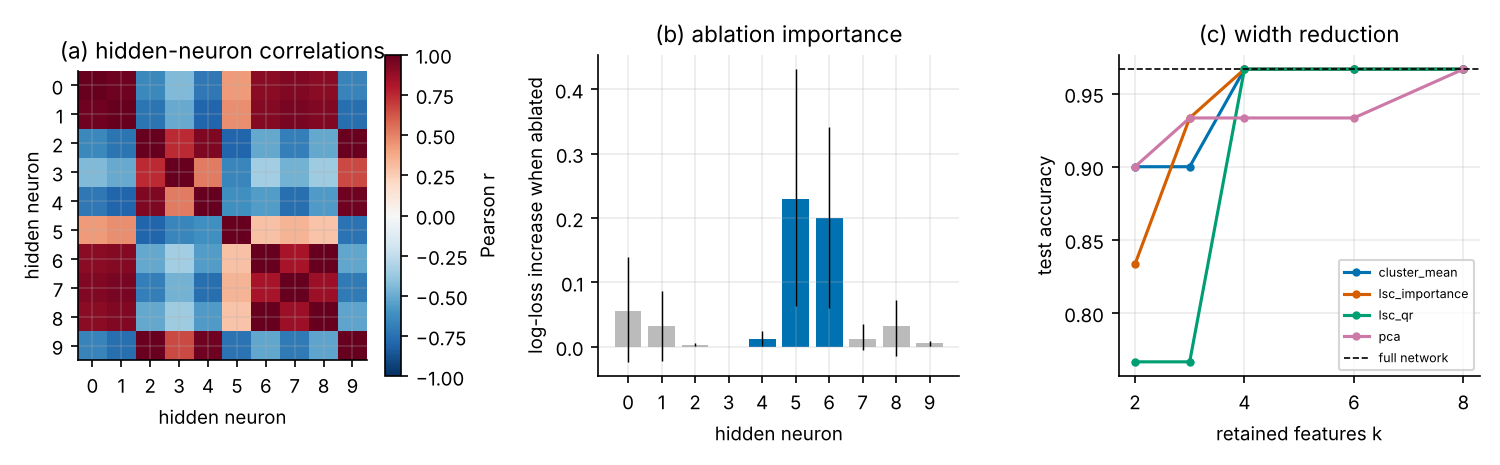
\includegraphics[width=\textwidth]{e5_iris.png}
\caption{Iris case study: (a) correlation of hidden neurons; (b) ablation importance with paired-bootstrap 95\% intervals (blue: adjusted $p<0.05$ and loss increase $\ge0.01$); (c) test accuracy of reduced models.}\label{fig:e5}\end{figure}
(i)~The accuracy intervals are wide for $n=30$ ($[0.833,0.994]$). (ii)~All neurons are associated with the response, but only $3/10$ (Iris) and $4/16$ (Breast Cancer) matter individually in the ablation test. (iii)~With the paired test all $30$ pairwise contrasts on Iris are significant; independent-sample Mann--Whitney tests flag $18$ raw and $16$ after Holm. (iv)~The surrogate head explains almost all deviance (McFadden $R^2\approx0.97$--$0.98$, whole-layer LR test $p<10^{-40}$), yet no Wald test and at most $1$ drop-one LR test is significant: the effective rank is $2.0$ of $10$ and $2.5$ of $16$, so neurons are nearly interchangeable and individual coefficients are not identified.

\subsection{E7: PyTorch networks on image data}\label{sec:e7}
To test whether these findings are an artefact of tiny one-hidden-layer networks, we trained PyTorch models on a 5000-image sample of MNIST (shipped with the \texttt{mlxtend} package; $70/30$ stratified split, 8 seeds): a three-hidden-layer MLP ($784\text{-}256\text{-}128\text{-}64\text{-}10$) and a small CNN (two convolution--pooling blocks, a $128$-unit dense layer). The adapter reads the last hidden layer through a forward hook. The audit (three seeds, $1500$ fit images) gives Table~\ref{tab:e7a}.
\begin{table}[ht]\centering\small
\caption{Audit of PyTorch models (mean over 3 seeds); ``dead'' means constant on the evaluation sample.}\label{tab:e7a}
\begin{tabular}{lrr}\toprule
 & deep MLP & CNN\\\midrule
Hidden units $k$ & 64 & 128\\
Test accuracy & 0.939 & 0.964\\
Effective rank & 7.6 & 11.4\\
Participation ratio & 6.0 & 7.4\\
Dead neurons & 10.7 & 44.7\\
Neurons associated with class (BH) & 52.7 & 81.3\\
Neurons with significant ablation effect (BH) & 0.0 & 1.0\\
\bottomrule\end{tabular}

\end{table}
The layers are of very low effective rank ($7.6$ of $64$; $11.4$ of $128$; participation ratios $6.0$ and $7.4$) and many units are dead on the evaluation sample ($10.7$ and $44.7$). Nearly all live neurons are associated with the class, but on average $0.0$ and $1.0$ neurons have a significant individual ablation effect: the network as a whole matters, individual units do not. This is the identifiability problem of Section~\ref{sec:e5} in deeper and larger networks. Compression results for the same models are in Table~\ref{tab:e7}.

\subsection{E6--E7: compensated pruning against published baselines}\label{sec:e6}
We compare LSC with the selection rule of Proposition~\ref{prop:bound} (LSC-QR, which uses neither labels nor the head), layer-wise OBS (greedy), ThiNet, data-free neuron merging, CUR-style leverage selection followed by LSC, a random subset followed by LSC (a control for the value of selection), magnitude pruning, and the cluster-mean and PCA reductions (which evaluate all $k$ neurons; marked $^\dagger$). Tabular data: Iris ($k{=}12$), Wine, Breast Cancer ($k{=}16$), Digits ($k{=}32$) and Diabetes (regression, $k{=}16$); one hidden layer; $15$ random $70/30$ splits; every reduction is built on the training activations and scored on the test set (Tables~\ref{tab:e6a}--\ref{tab:e6b}). Image data: the PyTorch models above (Table~\ref{tab:e7}).
\begin{table}[ht]\centering\small
\caption{Change relative to the full network (mean $\pm$ sd over 15 splits; accuracy points, $R^2$ points for Diabetes) at \textbf{50\%} of the width. Bold: best among methods that reduce the neurons computed. $^\dagger$ evaluates all $k$ neurons.}\label{tab:e6a}
\begin{tabular}{lrrrrr}\toprule
Method & iris & wine & breast cancer & digits & diabetes ($R^2$)\\\midrule
LSC-QR (label-free) & +0.1 $\pm$ 1.0 & \textbf{-0.4 $\pm$ 2.2} & -0.1 $\pm$ 0.8 & -2.8 $\pm$ 1.2 & -0.1 $\pm$ 1.7\\
OBS-greedy \cite{hassibi1993,dong2017} & -0.1 $\pm$ 0.6 & -1.1 $\pm$ 2.1 & -0.1 $\pm$ 0.5 & \textbf{-2.2 $\pm$ 1.2} & -0.2 $\pm$ 1.4\\
ThiNet \cite{luo2017} & -0.4 $\pm$ 3.2 & -1.4 $\pm$ 2.0 & \textbf{-0.0 $\pm$ 0.7} & -7.5 $\pm$ 2.5 & -2.7 $\pm$ 2.6\\
Neuron merging, data-free \cite{srinivas2015,kim2020} & -2.7 $\pm$ 9.3 & -2.1 $\pm$ 3.6 & \textbf{-0.0 $\pm$ 0.9} & -11.5 $\pm$ 3.2 & -9.2 $\pm$ 11.0\\
CUR leverage + LSC \cite{mahoney2009} & -0.0 $\pm$ 1.2 & -1.9 $\pm$ 3.8 & -0.2 $\pm$ 0.6 & -3.7 $\pm$ 1.2 & \textbf{+0.1 $\pm$ 3.2}\\
random subset + LSC & \textbf{+0.4 $\pm$ 2.8} & -3.0 $\pm$ 2.6 & -0.5 $\pm$ 0.9 & -4.7 $\pm$ 1.6 & -1.9 $\pm$ 3.1\\
weight-norm pruning \cite{han2015} & -11.0 $\pm$ 15.7 & -6.9 $\pm$ 6.9 & -0.7 $\pm$ 1.0 & -20.0 $\pm$ 4.5 & -109.0 $\pm$ 46.4\\
cluster-mean$^\dagger$ & -1.2 $\pm$ 3.6 & -0.5 $\pm$ 1.3 & -0.3 $\pm$ 0.9 & -2.2 $\pm$ 1.1 & -0.1 $\pm$ 0.9\\
PCA$^\dagger$ & +0.4 $\pm$ 2.3 & -0.5 $\pm$ 1.1 & -0.7 $\pm$ 0.7 & -0.5 $\pm$ 0.6 & -0.2 $\pm$ 1.4\\
\midrule
full network (metric) & 0.957 & 0.979 & 0.971 & 0.973 & 0.448\\
\bottomrule\end{tabular}

\end{table}
\begin{table}[ht]\centering\small
\caption{As Table~\ref{tab:e6a} at \textbf{25\%} of the width.}\label{tab:e6b}
\begin{tabular}{lrrrrr}\toprule
Method & iris & wine & breast cancer & digits & diabetes ($R^2$)\\\midrule
LSC-QR (label-free) & -1.0 $\pm$ 3.4 & -2.3 $\pm$ 3.6 & \textbf{-0.3 $\pm$ 0.8} & -13.6 $\pm$ 3.9 & -2.3 $\pm$ 4.1\\
OBS-greedy \cite{hassibi1993,dong2017} & \textbf{-0.4 $\pm$ 1.7} & \textbf{-2.0 $\pm$ 2.4} & -0.4 $\pm$ 0.8 & \textbf{-11.3 $\pm$ 1.9} & \textbf{-0.9 $\pm$ 2.6}\\
ThiNet \cite{luo2017} & -13.5 $\pm$ 11.6 & -7.9 $\pm$ 9.5 & -1.5 $\pm$ 1.7 & -31.9 $\pm$ 5.5 & -20.4 $\pm$ 10.3\\
Neuron merging, data-free \cite{srinivas2015,kim2020} & -16.4 $\pm$ 16.0 & -17.0 $\pm$ 12.4 & -4.7 $\pm$ 9.2 & -41.7 $\pm$ 6.3 & -79.8 $\pm$ 78.6\\
CUR leverage + LSC \cite{mahoney2009} & -2.2 $\pm$ 3.9 & -4.7 $\pm$ 5.2 & -2.2 $\pm$ 4.0 & -16.5 $\pm$ 4.8 & -9.2 $\pm$ 6.7\\
random subset + LSC & -12.3 $\pm$ 10.8 & -9.9 $\pm$ 8.9 & -2.1 $\pm$ 1.7 & -21.0 $\pm$ 5.1 & -5.5 $\pm$ 4.0\\
weight-norm pruning \cite{han2015} & -29.5 $\pm$ 14.3 & -16.3 $\pm$ 11.6 & -3.7 $\pm$ 5.9 & -41.1 $\pm$ 5.0 & -257.9 $\pm$ 79.3\\
cluster-mean$^\dagger$ & -0.1 $\pm$ 3.1 & -0.6 $\pm$ 1.5 & -0.3 $\pm$ 0.9 & -6.5 $\pm$ 2.1 & -0.1 $\pm$ 2.6\\
PCA$^\dagger$ & -0.1 $\pm$ 1.8 & -0.6 $\pm$ 1.1 & +0.2 $\pm$ 0.8 & -3.3 $\pm$ 1.6 & -0.5 $\pm$ 3.1\\
\midrule
full network (metric) & 0.957 & 0.979 & 0.971 & 0.973 & 0.448\\
\bottomrule\end{tabular}

\end{table}
\begin{table}[ht]\centering\small
\caption{PyTorch models on MNIST (8 seeds): change in test accuracy (points) relative to the full network.}\label{tab:e7}
\begin{tabular}{lrrrr}\toprule
 & \multicolumn{2}{c}{deep MLP ($k{=}64$)} & \multicolumn{2}{c}{CNN ($k{=}128$)}\\
Method & 50\% width & 25\% width & 50\% width & 25\% width\\\midrule
LSC-QR (label-free) & +0.0 $\pm$ 0.1 & -0.0 $\pm$ 0.1 & +0.0 $\pm$ 0.1 & -0.4 $\pm$ 0.1\\
OBS-greedy \cite{hassibi1993,dong2017} & \textbf{+0.0 $\pm$ 0.1} & \textbf{+0.0 $\pm$ 0.1} & \textbf{+0.0 $\pm$ 0.1} & \textbf{-0.3 $\pm$ 0.1}\\
ThiNet \cite{luo2017} & -0.2 $\pm$ 0.3 & -3.8 $\pm$ 1.6 & -0.2 $\pm$ 0.3 & -2.1 $\pm$ 0.8\\
Neuron merging, data-free \cite{srinivas2015,kim2020} & -0.5 $\pm$ 0.4 & -4.3 $\pm$ 3.5 & -0.3 $\pm$ 0.2 & -3.5 $\pm$ 1.3\\
CUR leverage + LSC \cite{mahoney2009} & +0.0 $\pm$ 0.2 & -0.2 $\pm$ 0.5 & \textbf{+0.0 $\pm$ 0.1} & -0.9 $\pm$ 0.4\\
random subset + LSC & -0.0 $\pm$ 0.2 & -0.6 $\pm$ 0.7 & -0.4 $\pm$ 0.2 & -2.0 $\pm$ 1.0\\
weight-norm pruning \cite{han2015} & -2.3 $\pm$ 1.5 & -10.9 $\pm$ 3.2 & -1.3 $\pm$ 1.0 & -17.3 $\pm$ 7.8\\
cluster-mean$^\dagger$ & -0.1 $\pm$ 0.2 & -0.4 $\pm$ 0.3 & -0.2 $\pm$ 0.3 & -0.6 $\pm$ 0.5\\
PCA$^\dagger$ & -0.0 $\pm$ 0.3 & -0.0 $\pm$ 0.3 & +0.1 $\pm$ 0.3 & +0.0 $\pm$ 0.3\\
\midrule
full network (test accuracy) & \multicolumn{2}{c}{0.943} & \multicolumn{2}{c}{0.969}\\
\bottomrule\end{tabular}

\end{table}
\paragraph{Findings.} (i)~Compensation is what matters. At half width, LSC-QR and OBS-greedy stay within about $1$ point of the full network except on Digits ($-2.8$, $-2.2$), and CUR+LSC within $2$ points except on Digits ($-3.7$); ThiNet loses $7.5$ points on Digits and $2.7$ $R^2$ points on Diabetes, neuron merging $11.5$ and $9.2$, and weight-norm pruning $20$ and $109$. On the CNN at a quarter of the width, LSC-QR loses $0.4$ points and OBS $0.3$, against $2.1$ for ThiNet, $3.5$ for neuron merging and $17.3$ for magnitude pruning; on the deep MLP LSC-QR loses $<0.1$ point at a quarter of the width. (ii)~Selection matters less than compensation at moderate compression -- the random subset with LSC is competitive at $50\%$ on Iris and Breast Cancer -- but matters at $25\%$: on Digits LSC-QR loses $13.6$ and OBS $11.3$ against $21.0$ for random selection. (iii)~OBS-greedy and LSC-QR are comparable at half width (LSC-QR is better on Wine, OBS on Digits) and OBS is better in the hardest settings (Digits at $25\%$, CNN at $25\%$), as expected from Proposition~\ref{prop:equiv}: it uses the same compensation but chooses the subset greedily with knowledge of the head. LSC-QR's advantage is not accuracy but that selection needs neither labels nor the head and costs a single pivoted QR. (iv)~Cluster-mean and PCA often lose less than subset methods at the same number of \emph{features}, but they evaluate all $k$ neurons, so they compress the head and not the computation. We performed no formal significance tests between methods; differences below one standard deviation should not be over-read.

\subsection{E8: the error bound}\label{sec:e8}
For Wine, Breast Cancer and Digits ($10$ splits each, widths $25$, $50$, $75\%$) we computed the training logit error of LSC-QR, the bound $\|W_P\|_2^2\|R_{22}\|_F^2/n$ of Proposition~\ref{prop:bound}, the test error, and the ratio of the QR residual energy $\|R_{22}\|_F^2$ to the Eckart--Young optimum $\sum_{i>m}\sigma_i^2$.
\begin{table}[ht]\centering\small
\caption{Medians over 10 splits. ``Bound/actual'': bound divided by the training logit error; ``rel.\ test error'': test logit error divided by the logit variance.}\label{tab:e8}
\begin{tabular}{llrrrrr}\toprule
Data & width & bound holds & bound/actual & QR/optimal & test/train & rel.\ test error\\\midrule
breast cancer & 25\% & 100\% & 6.9 & 1.38 & 1.03 & 0.024\\
breast cancer & 50\% & 100\% & 6.2 & 1.61 & 1.05 & 0.006\\
breast cancer & 75\% & 100\% & 3.6 & 1.69 & 1.13 & 0.001\\
digits & 25\% & 100\% & 2.8 & 1.60 & 1.00 & 0.258\\
digits & 50\% & 100\% & 2.8 & 1.79 & 1.05 & 0.082\\
digits & 75\% & 100\% & 2.3 & 1.89 & 1.20 & 0.025\\
wine & 25\% & 100\% & 4.6 & 1.42 & 1.01 & 0.079\\
wine & 50\% & 100\% & 4.1 & 1.64 & 1.20 & 0.020\\
wine & 75\% & 100\% & 2.5 & 1.74 & 1.36 & 0.005\\
\bottomrule\end{tabular}

\end{table}
The bound held in all $90$ cases, with slack of $2.3$--$6.9\times$; the test error is $1.00$--$1.36$ times the training error (the compensation does not overfit materially at these sample sizes); and plain pivoted QR is within $1.4$--$1.9\times$ of the optimum in residual energy. The bound is in-sample; we have no out-of-sample guarantee beyond this empirical behaviour.

\section{Discussion and limitations}
\textbf{Scope.} Contribution tests and compression act on the last hidden layer only; extending compensation across layers by propagating the regression through the next weight matrix is natural but not studied. \textbf{Evidence.} Experiments use scikit-learn and PyTorch models on small benchmarks; the image experiments use a 5000-image MNIST sample and a small CNN, not a large-scale backbone, and the IDC experiment of \cite{almohamad2024} was not reproduced. The PyTorch adapter was exercised in E7; the Keras adapter was not executed. The classical case studies use a single split. We did not run formal tests across methods. \textbf{Tests.} Ablation and permutation tests concern the \emph{fitted} network, not population effects. The per-neuron p-values are subject to the identifiability problem documented above; layer- or cluster-level tests are preferable. \textbf{Novelty.} Compensated pruning is not new (Section~\ref{sec:related}); we do not claim a new pruning algorithm, and in our experiments greedy OBS is comparable to LSC-QR and better in the hardest settings. \textbf{Authorship note.} The CLT-interval critique concerns a procedure proposed in an earlier paper of some of the present authors \cite{almohamad2024}; the conclusions here supersede its Algorithm~6 as an interval for accuracy.

\section{Conclusion}
A trained network can be audited statistically, but the audit must use intervals with the right target, multiplicity control and awareness of what the data can identify. For a fixed network, accuracy intervals should be Wilson/Clopper--Pearson or test-set bootstrap; the CLT interval over bootstrap replicates covers the true accuracy with probability $2F_{B-1}(t/\sqrt{B+1})-1$, far below nominal. Trained hidden layers are close to low-dimensional, which limits per-neuron inference and explains why least-squares compensated pruning, which OBS, ThiNet's reconstruction and our label-free QR selector all instantiate, removes half to three quarters of the units of the last hidden layer at small cost.

\section*{Data and code availability}
Data sets are scikit-learn benchmarks and the 5000-image MNIST sample from \texttt{mlxtend}. The package \texttt{annstat}, its tests and the scripts reproducing every table and figure are provided with this manuscript (MIT licence).

\section*{Declarations}
\noindent\textbf{Author contributions, funding, competing interests:} to be completed by the authors before submission.

\appendix
\section{Proofs}\label{app:proofs}
\begin{proof}[Proof of Proposition~\ref{prop:clt}]
Put $\sigma_n^2=\theta(1-\theta)/n$, $Z_n=(\hat p-\theta)/\sigma_n$ and $U_b=(a_b-\hat p)/\sigma_n$, $b=1,\dots,B$. By the de Moivre--Laplace theorem $Z_n\to N(0,1)$ in distribution. Conditionally on $\hat p$ the $U_b$ are i.i.d.\ with mean $0$ and variance $\hat p(1-\hat p)/(\theta(1-\theta))\to1$ in probability, and by the Lindeberg--Feller theorem (applied conditionally, with $\hat p\to\theta\in(0,1)$ in probability) $E[e^{i\,u^\top U}\mid\hat p]\to e^{-\|u\|^2/2}$ in probability for every $u\in\R^B$. Hence for $v\in\R$, $u\in\R^B$, $E\big[e^{ivZ_n}E[e^{iu^\top U}\mid \hat p]\big]\to e^{-v^2/2-\|u\|^2/2}$, so $(Z_n,U)\to(Z,\xi)$ in distribution with $Z\sim N(0,1)$ and $\xi\sim N(0,I_B)$ independent. The event $\{\theta\in I\}$ is $\{|\bar a-\theta|\le t\,s/\sqrt B\}$ with $t=t_{B-1,1-\alpha/2}$; dividing by $\sigma_n$ and using $\bar a-\theta=\sigma_n(Z_n+\bar U)$ and $s=\sigma_nS_U$ (sample standard deviation of $U$), it equals $\{|Z_n+\bar U|\le t\,S_U/\sqrt B\}$, a continuous function of $(Z_n,U)$ whose boundary has probability zero under the limit law. By the portmanteau theorem the coverage converges to $\Pr(|Z+\bar\xi|\le t\,S_\xi/\sqrt B)$. Now $Z+\bar\xi\sim N(0,1+1/B)$ is independent of $S_\xi^2\sim\chi^2_{B-1}/(B-1)$ (independence of $\bar\xi$ and $S_\xi$ for Gaussian samples, and of $Z$), so $(Z+\bar\xi)/(\sqrt{1+1/B}\,S_\xi)\sim t_{B-1}$ and
\[
\Pr\!\Big(|Z+\bar\xi|\le \tfrac{t\,S_\xi}{\sqrt B}\Big)=\Pr\!\Big(|t_{B-1}|\le\tfrac{t}{\sqrt{B(1+1/B)}}\Big)=2F_{B-1}\!\Big(\tfrac{t}{\sqrt{B+1}}\Big)-1.
\]
As $B\to\infty$, $t_{B-1,1-\alpha/2}\to z_{1-\alpha/2}$ and $z/\sqrt{B+1}\to0$, so the limit tends to $0$; the limit decreases over the tabulated values $B=2,\dots,1000$ (checked numerically).
\end{proof}

\begin{proof}[Proof of Proposition~\ref{prop:equiv}]
(b) Regressing $Z=[\mathbf 1\;H_S\;H_P][b^\top;W_S;W_P]$ on $A=[\mathbf 1\;H_S]$ gives $(A^\top A)^{-1}A^\top Z=[b^\top;W_S]+\hat B W_P$, i.e.\ \eqref{eq:lsc}; the minimiser is unique since $A$ has full column rank.
(a) Let $S$ index the rows of $\Theta$ allowed to be non-zero (always containing the intercept), $\Theta^{(S)}$ the minimiser of $L(\Theta)=\|A_k(\Theta-\Theta_0)\|_F^2$ over $\{\Theta:\text{rows}\notin S\text{ are }0\}$, and $M_S$ the inverse of $G_S$ (principal submatrix of $G$) padded by zeros. Initially $S$ is everything, $\Theta^{(S)}=\Theta_0$, $M_S=G^{-1}$. Within the subspace the objective is quadratic with Hessian $G_S$ and minimiser $\Theta^{(S)}$, so the minimiser with the further constraint that row $j$ vanishes is, by the Lagrange condition, $\Theta^{(S)}-M_Se_je_j^\top\Theta^{(S)}/(M_S)_{jj}$, which is the OBS update. The block-elimination identity $(G_{S\setminus j})^{-1}=(G_S^{-1})_{S\setminus j,S\setminus j}-(G_S^{-1})_{S\setminus j,j}(G_S^{-1})_{j,S\setminus j}/(G_S^{-1})_{jj}$ is exactly the Hessian-inverse update used by OBS. By induction after any sequence the iterate is the constrained minimiser for the current $S$, which by (b) is \eqref{eq:lsc}.
(c) $\mathrm{diag}(s)W_S$ with unchanged $b$ is a particular affine head on $H_S$; by (b) the least-squares head has a logit error no larger.
\end{proof}

\begin{proof}[Proof of Proposition~\ref{prop:bound}]
By Proposition~\ref{prop:equiv}(b), $Z'=A[b'^\top;W']$ and $Z-Z'=(H_P-A\hat B)W_P=RW_P$, so $\|Z-Z'\|_F\le\|R\|_F\|W_P\|_2$. Regression on $[\mathbf 1\;H_S]$ is regression of $\tilde H_P$ on $\tilde H_S$ after centring, hence $R=(I-Q_1Q_1^\top)\tilde H_P$ with $Q_1$ the first $m$ columns of $Q$ (an orthonormal basis of $\mathrm{span}(\tilde H_S)$ when the first $m$ pivots are $S$). From $\tilde H_P=Q_1R_{12}+Q_2R_{22}$ we get $R=Q_2R_{22}$ and $\|R\|_F=\|R_{22}\|_F$. Next, $\tilde H=QR_QP^\top$ has the same singular values as $R_Q$, and $R_Q$ differs from the matrix $[R_{11}\;R_{12};\,0\;0]$, which has rank at most $m$, exactly by the block $R_{22}$; by Eckart--Young \cite{eckart1936}, $\|R_{22}\|_F^2\ge\sum_{i>m}\sigma_i^2(R_Q)=\sum_{i>m}\sigma_i^2(\tilde H)$. The strong RRQR statement is Theorem~3.2 of \cite{gu1996}: $\sigma_j(R_{22})\le\sqrt{1+f^2m(k-m)}\,\sigma_{m+j}(\tilde H)$; square and sum over $j$.
\end{proof}

\begin{thebibliography}{99}\small
\bibitem{aghajanyan2021} Aghajanyan, A., Gupta, S., Zettlemoyer, L. (2021). Intrinsic dimensionality explains the effectiveness of language model fine-tuning. \emph{Proc.\ ACL-IJCNLP}.
\bibitem{aghasi2017} Aghasi, A., Abdi, A., Nguyen, N., Romberg, J. (2017). Net-Trim: convex pruning of deep neural networks with performance guarantee. \emph{Advances in Neural Information Processing Systems} 30.
\bibitem{agresti1998} Agresti, A., Coull, B.A. (1998). Approximate is better than ``exact'' for interval estimation of binomial proportions. \emph{The American Statistician} 52, 119--126.
\bibitem{albert1984} Albert, A., Anderson, J.A. (1984). On the existence of maximum likelihood estimates in logistic regression models. \emph{Biometrika} 71, 1--10.
\bibitem{almohamad2024} Al-Mohamad, M.Y., Bevrani, H., Haydari, A.A. (2024). Statistical tuning of artificial neural network. arXiv:2409.16426.
\bibitem{angelopoulos2023} Angelopoulos, A.N., Bates, S. (2023). Conformal prediction: a gentle introduction. \emph{Foundations and Trends in Machine Learning} 16, 494--591.
\bibitem{ansuini2019} Ansuini, A., Laio, A., Macke, J.H., Zoccolan, D. (2019). Intrinsic dimension of data representations in deep neural networks. \emph{Advances in Neural Information Processing Systems} 32.
\bibitem{bates2023} Bates, S., Hastie, T., Tibshirani, R. (2024). Cross-validation: what does it estimate and how well does it do it? \emph{Journal of the American Statistical Association} 119, 1434--1445.
\bibitem{benavoli2017} Benavoli, A., Corani, G., Dem\v{s}ar, J., Zaffalon, M. (2017). Time for a change: a tutorial for comparing multiple classifiers through Bayesian analysis. \emph{Journal of Machine Learning Research} 18(77), 1--36.
\bibitem{bengio2004} Bengio, Y., Grandvalet, Y. (2004). No unbiased estimator of the variance of $K$-fold cross-validation. \emph{Journal of Machine Learning Research} 5, 1089--1105.
\bibitem{benjamini1995} Benjamini, Y., Hochberg, Y. (1995). Controlling the false discovery rate: a practical and powerful approach to multiple testing. \emph{Journal of the Royal Statistical Society B} 57, 289--300.
\bibitem{benjamini2001} Benjamini, Y., Yekutieli, D. (2001). The control of the false discovery rate in multiple testing under dependency. \emph{Annals of Statistics} 29, 1165--1188.
\bibitem{blalock2020} Blalock, D., Gonzalez Ortiz, J.J., Frankle, J., Guttag, J. (2020). What is the state of neural network pruning? \emph{Proceedings of Machine Learning and Systems} 2.
\bibitem{breiman2001} Breiman, L. (2001). Random forests. \emph{Machine Learning} 45, 5--32.
\bibitem{brown2001} Brown, L.D., Cai, T.T., DasGupta, A. (2001). Interval estimation for a binomial proportion. \emph{Statistical Science} 16, 101--133.
\bibitem{businger1965} Businger, P., Golub, G.H. (1965). Linear least squares solutions by Householder transformations. \emph{Numerische Mathematik} 7, 269--276.
\bibitem{candes2018} Cand\`es, E., Fan, Y., Janson, L., Lv, J. (2018). Panning for gold: ``model-X'' knockoffs for high dimensional controlled variable selection. \emph{Journal of the Royal Statistical Society B} 80, 551--577.
\bibitem{clopper1934} Clopper, C.J., Pearson, E.S. (1934). The use of confidence or fiducial limits illustrated in the case of the binomial. \emph{Biometrika} 26, 404--413.
\bibitem{davison1997} Davison, A.C., Hinkley, D.V. (1997). \emph{Bootstrap Methods and their Application}. Cambridge University Press.
\bibitem{demsar2006} Dem\v{s}ar, J. (2006). Statistical comparisons of classifiers over multiple data sets. \emph{Journal of Machine Learning Research} 7, 1--30.
\bibitem{denil2013} Denil, M., Shakibi, B., Dinh, L., Ranzato, M., de Freitas, N. (2013). Predicting parameters in deep learning. \emph{Advances in Neural Information Processing Systems} 26.
\bibitem{dietterich1998} Dietterich, T.G. (1998). Approximate statistical tests for comparing supervised classification learning algorithms. \emph{Neural Computation} 10, 1895--1923.
\bibitem{dong2017} Dong, X., Chen, S., Pan, S.J. (2017). Learning to prune deep neural networks via layer-wise optimal brain surgeon. \emph{Advances in Neural Information Processing Systems} 30.
\bibitem{eckart1936} Eckart, C., Young, G. (1936). The approximation of one matrix by another of lower rank. \emph{Psychometrika} 1, 211--218.
\bibitem{efron1979} Efron, B. (1979). Bootstrap methods: another look at the jackknife. \emph{Annals of Statistics} 7, 1--26.
\bibitem{efron1997} Efron, B., Tibshirani, R. (1997). Improvements on cross-validation: the .632+ bootstrap method. \emph{Journal of the American Statistical Association} 92, 548--560.
\bibitem{firth1993} Firth, D. (1993). Bias reduction of maximum likelihood estimates. \emph{Biometrika} 80, 27--38.
\bibitem{fisher2019} Fisher, A., Rudin, C., Dominici, F. (2019). All models are wrong, but many are useful: learning a variable's importance by studying an entire class of prediction models simultaneously. \emph{Journal of Machine Learning Research} 20(177), 1--81.
\bibitem{frankle2019} Frankle, J., Carbin, M. (2019). The lottery ticket hypothesis: finding sparse, trainable neural networks. \emph{International Conference on Learning Representations}.
\bibitem{frantar2022} Frantar, E., Alistarh, D. (2022). Optimal Brain Compression: a framework for accurate post-training quantization and pruning. \emph{Advances in Neural Information Processing Systems} 35.
\bibitem{frantar2023} Frantar, E., Alistarh, D. (2023). SparseGPT: massive language models can be accurately pruned in one-shot. \emph{Proceedings of the 40th International Conference on Machine Learning}, PMLR 202.
\bibitem{friedman1937} Friedman, M. (1937). The use of ranks to avoid the assumption of normality implicit in the analysis of variance. \emph{Journal of the American Statistical Association} 32, 675--701.
\bibitem{garson1991} Garson, G.D. (1991). Interpreting neural-network connection weights. \emph{AI Expert} 6(4), 46--51.
\bibitem{gu1996} Gu, M., Eisenstat, S.C. (1996). Efficient algorithms for computing a strong rank-revealing QR factorization. \emph{SIAM Journal on Scientific Computing} 17, 848--869.
\bibitem{han2015} Han, S., Pool, J., Tran, J., Dally, W.J. (2015). Learning both weights and connections for efficient neural networks. \emph{Advances in Neural Information Processing Systems} 28.
\bibitem{hassibi1993} Hassibi, B., Stork, D.G. (1993). Second order derivatives for network pruning: Optimal Brain Surgeon. \emph{Advances in Neural Information Processing Systems} 5.
\bibitem{hauck1977} Hauck, W.W., Donner, A. (1977). Wald's test as applied to hypotheses in logit analysis. \emph{Journal of the American Statistical Association} 72, 851--853.
\bibitem{he2017} He, Y., Zhang, X., Sun, J. (2017). Channel pruning for accelerating very deep neural networks. \emph{Proceedings of the IEEE International Conference on Computer Vision}.
\bibitem{hoefler2021} Hoefler, T., Alistarh, D., Ben-Nun, T., Dryden, N., Peste, A. (2021). Sparsity in deep learning: pruning and growth for efficient inference and training in neural networks. \emph{Journal of Machine Learning Research} 22(241), 1--124.
\bibitem{holm1979} Holm, S. (1979). A simple sequentially rejective multiple test procedure. \emph{Scandinavian Journal of Statistics} 6, 65--70.
\bibitem{hooker2021} Hooker, G., Mentch, L., Zhou, S. (2021). Unrestricted permutation forces extrapolation: variable importance requires at least one more model, or there is no free variable importance. \emph{Statistics and Computing} 31, 82.
\bibitem{horel2020} Horel, E., Giesecke, K. (2020). Significance tests for neural networks. \emph{Journal of Machine Learning Research} 21(227), 1--29.
\bibitem{hu2022} Hu, E.J., Shen, Y., Wallis, P., Allen-Zhu, Z., Li, Y., Wang, S., Wang, L., Chen, W. (2022). LoRA: low-rank adaptation of large language models. \emph{International Conference on Learning Representations}.
\bibitem{kim2020} Kim, W., Kim, S., Park, M., Jeon, G. (2020). Neuron merging: compensating for pruned neurons. \emph{Advances in Neural Information Processing Systems} 33.
\bibitem{kornblith2019} Kornblith, S., Norouzi, M., Lee, H., Hinton, G. (2019). Similarity of neural network representations revisited. \emph{Proceedings of the 36th International Conference on Machine Learning}, PMLR 97.
\bibitem{kruskal1952} Kruskal, W.H., Wallis, W.A. (1952). Use of ranks in one-criterion variance analysis. \emph{Journal of the American Statistical Association} 47, 583--621.
\bibitem{lecun1990} LeCun, Y., Denker, J.S., Solla, S.A. (1990). Optimal brain damage. \emph{Advances in Neural Information Processing Systems} 2.
\bibitem{lei2018} Lei, J., G'Sell, M., Rinaldo, A., Tibshirani, R.J., Wasserman, L. (2018). Distribution-free predictive inference for regression. \emph{Journal of the American Statistical Association} 113, 1094--1111.
\bibitem{li2017} Li, H., Kadav, A., Durdanovic, I., Samet, H., Graf, H.P. (2017). Pruning filters for efficient convnets. \emph{International Conference on Learning Representations}.
\bibitem{lundberg2017} Lundberg, S.M., Lee, S.-I. (2017). A unified approach to interpreting model predictions. \emph{Advances in Neural Information Processing Systems} 30.
\bibitem{luo2017} Luo, J.-H., Wu, J., Lin, W. (2017). ThiNet: a filter level pruning method for deep neural network compression. \emph{Proceedings of the IEEE International Conference on Computer Vision}.
\bibitem{mahoney2009} Mahoney, M.W., Drineas, P. (2009). CUR matrix decompositions for improved data analysis. \emph{Proceedings of the National Academy of Sciences} 106, 697--702.
\bibitem{mann1947} Mann, H.B., Whitney, D.R. (1947). On a test of whether one of two random variables is stochastically larger than the other. \emph{Annals of Mathematical Statistics} 18, 50--60.
\bibitem{molchanov2017} Molchanov, P., Tyree, S., Karras, T., Aila, T., Kautz, J. (2017). Pruning convolutional neural networks for resource efficient inference. \emph{International Conference on Learning Representations}.
\bibitem{molchanov2019} Molchanov, P., Mallya, A., Tyree, S., Frosio, I., Kautz, J. (2019). Importance estimation for neural network pruning. \emph{Proceedings of the IEEE/CVF Conference on Computer Vision and Pattern Recognition}.
\bibitem{nadeau2003} Nadeau, C., Bengio, Y. (2003). Inference for the generalization error. \emph{Machine Learning} 52, 239--281.
\bibitem{olden2002} Olden, J.D., Jackson, D.A. (2002). Illuminating the ``black box'': a randomization approach for understanding variable contributions in artificial neural networks. \emph{Ecological Modelling} 154, 135--150.
\bibitem{raghu2017} Raghu, M., Gilmer, J., Yosinski, J., Sohl-Dickstein, J. (2017). SVCCA: singular vector canonical correlation analysis for deep learning dynamics and interpretability. \emph{Advances in Neural Information Processing Systems} 30.
\bibitem{ribeiro2016} Ribeiro, M.T., Singh, S., Guestrin, C. (2016). ``Why should I trust you?'': explaining the predictions of any classifier. \emph{Proceedings of the 22nd ACM SIGKDD Conference}.
\bibitem{roy2007} Roy, O., Vetterli, M. (2007). The effective rank: a measure of effective dimensionality. \emph{Proceedings of the 15th European Signal Processing Conference (EUSIPCO)}.
\bibitem{shah2020} Shah, R.D., Peters, J. (2020). The hardness of conditional independence testing and the generalised covariance measure. \emph{Annals of Statistics} 48, 1514--1538.
\bibitem{srinivas2015} Srinivas, S., Babu, R.V. (2015). Data-free parameter pruning for deep neural networks. \emph{Proceedings of the British Machine Vision Conference (BMVC)}.
\bibitem{tomczak2014} Tomczak, M., Tomczak, E. (2014). The need to report effect size estimates revisited. \emph{Trends in Sport Sciences} 21, 19--25.
\bibitem{white2001} White, H., Racine, J. (2001). Statistical inference, the bootstrap, and neural-network modeling with application to foreign exchange rates. \emph{IEEE Transactions on Neural Networks} 12, 657--673.
\bibitem{wilcoxon1945} Wilcoxon, F. (1945). Individual comparisons by ranking methods. \emph{Biometrics Bulletin} 1, 80--83.
\bibitem{williams2001} Williams, C.K.I., Seeger, M. (2001). Using the Nystr\"om method to speed up kernel machines. \emph{Advances in Neural Information Processing Systems} 13.
\bibitem{wilson1927} Wilson, E.B. (1927). Probable inference, the law of succession, and statistical inference. \emph{Journal of the American Statistical Association} 22, 209--212.
\end{thebibliography}
\end{document}
